\chapter{Independent set color formulation for packing coloring}

\section{Introduction}

This chapter focuses on an adaptation of the independent set formulation for the PC problem. Firstly, Section \ref{sec:Stableformu} explains the idea and presents the new formulation. Then, Section \ref{sec:Stableimpl} describes the implementation. Section \ref{sec:Stableres} presents computational results and their interpretation. Finally, Section \ref{sec:StableBP} presents a new way to solve the formulation using standard branch and price algorithm.

\section{Formulation}
\label{sec:Stableformu}

\subsection{Idea}
As \hyperref[IC]{before}, there is one variable per independent set. Nevertheless, a specific independent set cannot be used for any color. Therefore, the set of independent set $I$ is divided in classes as represented in Figure \ref{fig:classeI}. The class $I_j$ is the set of independent sets that can be used for colors $1,2,\dots,j$ and not colors $> j$. The $\infty$ class can be used for any color due to the lack of path between its vertices. There is $D$ classes with $D$ the diameter because the distance between 2 connected vertices cannot exceed $D$ thus $I_j$ with $j\geq D$ is empty. For each class, we limit ourselves to the maximal sets. \\

\begin{mydef}
	\label{def:stableMax}
	A set of vertices $S$ belonging to class $I_j$ is \keyword{maximal} $\iff$ $\forall v \in V, S \cup v \notin I_j$.
\end{mydef}

\begin{figure}[H]
  \centering
  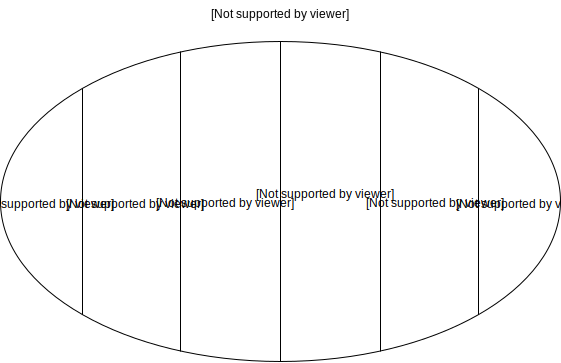
\includegraphics[scale=0.6]{figures/StableClass.png}
  %\def\svgwidth{\columnwidth}
  %\input{figures/StableClass.pdf_tex}
  \caption{Class separation of $I$}
  \label{fig:classeI}
\end{figure}

\subsection{Formulation}

The formulation denoted IPC need several variables and parameters which are the following : \\

\[ \forall i \in I\ x_{i} =
  \begin{cases}
    1       & \quad \text{if the independent set $i$ is taken to represent a color}  \\
    0  		& \quad \text{otherwise }\\
  \end{cases}
\]

As said, there is one variable by set. But some parameters are needed to complete the formulation. First, we need to know in which class are each set which was not needed for IC due to the non differentiation of colors. The classification is done in pre-processing as explained later in \ref{sec:Stableimpl}. Moreover, the content of each set as to be known like in IC. These are given by parameters denoted respectively $d$ and $c$.

\begin{comment}
\[ \forall i \in I, \forall k \in [1;D]\ d_{i,k} =
  \begin{cases}
    1       & \quad \text{if the independent set $i$ is in class $I_{k}$}  \\
    0  		& \quad \text{otherwise }\\
  \end{cases}
\]
\end{comment}


The class  of a independent set $i$ is $d_i$.

\[ \forall i \in I, \forall v \in V\ c_{iv} =
  \begin{cases}
    1       & \quad \text{if the vertex v is in the independent set $i$}  \\
    0  		& \quad \text{otherwise }\\
  \end{cases}
\]

All parameters and variables are defined so we can present the formulation :

\begin{eqnarray}
minimize\ &  \displaystyle\sum_{i \in I} x_i & \label{IPC:FE}\\
subject\ to &   \displaystyle\sum_{i \in I | v \in i}{x_{i}} = 1   & \forall v \in V  \label{IPC:C1}\\
			&   \displaystyle\sum_{i \in I | d_{i} \leq k }{x_{i}} \leq k    & \forall k \in [1;D-1]  \label{IPC:C2}\\
&  x_{i} \in \mathbb{B} &  \forall i \in I
\end{eqnarray}

The objective function \ref{IPC:FE} minimizes the number of independent set chosen thus the number of color. Each vertex is in one and only one chosen independent set so has a clearly defined color is fixed by Constraint \ref{IPC:C1}. Note that these two constraints are identical to the classical version of this formulation. Constraint \ref{IPC:C2} represents the fact that we cannot take too much sets from each partition. Indeed, we can take at most $j$ element from $I_j$ because they can be used only for color $1$ to $j$. We must also take into account the number of element taken from class lower than $I_j$. For example, if two elements from $I_2$ have already been taken in a partial solution then at most two elements of $I_4$ could be in the complete solution because colors 1 and 2 are already represented by $I_2$ thus $I_4$ can only take color 3 and 4.\\

Compared to IC, IPC has the same number of variable but the number of constraints increases from $N$ to $N+D$ which is still in $\mathbb{O}(N)$.

\section{Implementation}
\label{sec:Stableimpl}

IPC needs some pre-processing including finding all independent set and classifying them. All independent set are found by a classic backtracking generating all binary string of size $N$ representing which vertex is taken in the set. A branch can be pruned if we add a vertex sharing an edge with one of the vertices from the current independent set which make it loses its independent property by definition. Another case is when an independent set is not maximal. It is the case where we can add a vertex by keeping an independent set with the same Class. Each solution and its class is stored on a binary file to save space. This file is used as input for the "optimization" part/module of the code. This separation is used to make each part independent in term of code and memory usage. The optimization part is implemented with cplex library in c++. The choose of cplex over other possibilities like xpress or NEOS server is based on the price, size of instances\footnote{limitatioçn in free version}, compatibility with OS and integration in programming language. The pre-processing part is in $\mathbb{O}(2^N + N^2) = \mathbb{O}(2^N) $ due to exponential complexity of backtracking. In practice it can be much less due to pruning's efficiency being inversely proportional to the density of the graph. The algorithm used to solve a formulation is simply using the method solve from Cplex as black box. \\

\section{Result}
\label{sec:Stableres}

The algorithm was tested on instances from DIMACS for graph coloring encoded in .col format found \url{http://mat.gsia.cmu.edu/COLOR/instances.html}. We tested two formulations : the presented in \cite{PCModel} and the one presented in Section \ref{sec:Stableformu}. The hardware and software configuration on which the tests were conducted has as characteristic  :

\begin{itemize}
\item OS : Linux mint 18.1 (kernel 4.4.0).
\item CPU : Intel(R) Core(TM) i7-7700K CPU @ 4.20GHz with 4 cores ( 8 threads).
\item RAM : 32GB at 2400 MHz + 4GB of swap partition.
\item Secondary memory : SSD 120GB 
\item Cplex 12.7 with default parameters.
\end{itemize}

The results are represented on Table \ref{tbl:cpIS}. The preprocessing time for VC is not indicated because it is only a parser and take less than one ms which is negligible in comparison of the total time.
% In this table, \textcolor{red}{ERROR} represents the fact that the program ran out of RAM

\begin{table}[H]
\centering
\begin{tabular}{|c|c|c|c|c|c|c|}
\hline
Name & N & density  & time VC$\prime$ (s) & Pre-Time IS (s) & Time IS (s) & \# color\\
\hline
DSJC125.5 & 125 & 0.5 &   0.965143 &  0.930401  & 0.213191 & 116 \\
\hline
DSJC125.9 & 125 & 0.9 &  0.946579 & 0.008601 & 0.003331 & 122 \\
\hline
DSJC250.5 & 250 & 0.5 & 74.786779  & 102.042875  & 9.934149 & 239\\ 
\hline
DSJC250.9 & 250 & 0.9 &  10.150312 & 0.094591 & 0.020786 & 246 \\
\hline
DSJC500.9 & 500 & 0.9 &  45.448983 & 1.579720 & 0.074801 & 496  \\
\hline
DSJC1000.9 & 1000 & 0.9 &  735.636395 & 38.864877 & 1.069712 & 995  \\
\hline
flat300 20 & 300 & 0,2375 &  162.278250 & 796.447398 & 140.888260 & 286 \\
\hline
flat300 26 & 300 & 0.24  &  319.709602 & 620.181133 & 54.438221 & 289 \\
\hline
flat300 28 & 300 & 0.241 &  260.156268 & 602.066899 & 58.223397 & 289 \\
\hline
Latin square 10 & 900 & 0,38 &  39.507431 & 523.119600 & 0.347178 & 891 \\
\hline
\end{tabular}
\caption{Computation time per instances for two formulations}
\label{tbl:cpIS}
\end{table}

We can observe that it takes much longer time for preprocessing than solving for the IS formulation. Preprocessing time changes proportionally with N and inversely proportionally with density. On one hand, there is generally more independent set/subset when N increases with same density. On the other hand, a higher density means more edges thus less independent set. The density has a bigger impact than N on the time. For instance, going from 250 to 500 vertices with a density of 0.9 multiplies only the time by 3 but keeping 250 vertices and going from 0.9 to 0.5  multiply the time by nearly 1000 times. For VC formulations, the most important factor is N because there is $N^2$ variables. A higher density decreases the time but less than for IS. It can be explained by the lower number of constraint because there are more adjacent vertices which only need to not both have the color one. The density has less impact due to the fact that the number of variables is constant and the reduction in cardinality of constraint is nothing compared to the reduction of variables in IS.

The preprocessing time increases exponentially with $N$ but the cplex time is lower than the $VC\prime$ formulation

\section{Branch and Price}
\label{sec:StableBP}
\subsection{Introduction}

A big percentage of computation time is used on preprocessing and the solver time is lower than $VC\prime$ so can we reduce time by using the same formulation ? Indeed, it is the case, a way to reduce it is by using the column generation method. This general algorithm is often uses when dealing with problem having a large number of variables. 

\subsection{Algorithm}

The algorithm follows this structure : 
\newline

\begin{enumerate}
\item Solve linear relaxation master problem with restricted columns.
\item Get optimal dual value $\pi$.
\item Solve subproblem with coefficient $\pi$.
\item Add Column from subproblem to main problem.
\item Repeat until subproblem solution $\leq 0$. 
\end{enumerate}

This template introduces new concepts. Firstly, the idea of adding column which represents variable. The idea is to add a variable at each turn until the solution is optimal which means here that considering new independent sets will not improve the solution (coloring) quality. If we add column then all columns are not included initially. Indeed, we talk about \textbf{restricted} master problem. We start with a initial set of columns from which a solution exists. The master problem is the problem to solve. Generally; it has a variable for each solution from the initial problem. For instance, there can be a variable for each subset of location for the facility location problem which include a exponential number of variable which needs a lot of resource (memory, time,...) to be solved. In our case, we have to select several variables to have a solution but te number of variables is still exponential to N.

We solve the \textbf{linear relaxation} which means that each variable is considered as a real value instead of integer/boolean ones in order to have the dual variable coefficient $\pi$ and be able to compute reduced costs of the missing columns. Nonetheless, it would be inefficient to computed the reduced cost for all missing columns because we would need to enumerate all columns so all independent set which is equivalent to the preprocessing which we want to eliminate. As result, the choice of the new column is expressed as a MIP\footnote{Mixed Integer Problem} called subproblem which tends to minimize the reduced cost. This problem can also have constraints to ensure integrity of the new column. In our problem the new column must be an independent set.\\

\subsection{Implementation}

The section presents the different elements of branch and price adapted to our problem and formulation IS. First, we describe the  subproblem with the dual of linear relaxation of the master problem.
\begin{description}
\item[Master problem]

\begin{itemize}
	\item The matrix $d$ description : 
	\[ \forall i \in I, \forall k \in [1;D]\ d_{ik} =
	\begin{cases}
	1       & \quad \text{if the independent set $i$ is in $\bigcup_{j=1}^{k}$ $I_{j}$}  \\
	0  		& \quad \text{otherwise }\\
	\end{cases}
	\]
	\item  $I_{R}$ is the restricted set of columns.
\end{itemize}

\begin{align}
minimize\   &  \displaystyle\sum_{i \in I} x_i &  & \label{IPCD:FE}\\
subject\ to &   \displaystyle\sum_{i \in I }{c_{iv} x_{i}} = 1   & \forall v \in V\  & (\pi_v) \label{IPCD:C1}\\
			&   \displaystyle\sum_{i \in I_k}{d_{ik}x_{i}} \leq k   & \forall k \in [1;D-1]\ & (\alpha_k) \label{IPCD:C2}\\
&  x_{i} \in \mathbb{R} &  \forall i \in I_{R}
\end{align}



\item[Dual]
\begin{align}
maximize\   &  \displaystyle\sum_{v \in V} \pi_v + \displaystyle\sum_{k=1}^{D-1} k \alpha_k   &   \label{ISD:FE}\\
subject\ to &  \displaystyle\sum_{v \in V} c_{iv}\ \pi_v + \displaystyle\sum_{k=1}^{D-1} d_{ik} \alpha_k \leq 1 & \forall i \in I_{R}\label{ISD:C1}\\
&  \pi_{v} \in \mathbb{R} &  \forall v \in V \\ 
&  \alpha_{k} \in \mathbb{R} &  \forall k \in [1;D-1] \\ 
\end{align}
This gives us a reduced cost to minimize :
\[1 - \displaystyle\sum_{v \in V} c_{iv}\ \overline{\pi_v} - \displaystyle\sum_{k=1}^{D-1} d_{ik} \overline{\alpha_k} \text{ with $\overline{x}$ means the optimal value of x}\]

\item[Subproblem]
\begin{align}
maximize\   &  \displaystyle\sum_{v \in V} y_{v}\ \overline{\pi_v} + \displaystyle\sum_{k=1}^{D-1} z_{k} \overline{\alpha_k}   &   \label{ISSB:FE}\\
subject\ to\ & z_k \geq  z_{k+1} & \forall k \in [1;D-2]  \label{ISSB:C1} \\ 
& x_{uvk}  \leq y_u & \forall u,v \in V^{2}, \forall k \in [1;D-1] \label{ISSB:C2} \\
& x_{uvk}  \leq z_k & \forall u,v \in V^{2}, \forall k \in [1;D-1] \label{ISSB:C3} \\
& y_u + y_v + z_k - 2 \leq x_{uvk}  & \forall u,v \in V^{2}, \forall k \in [1;D-1] \label{ISSB:C4} \\
%&  x_{uvk} (k+1)  \leq  d_{uv} x_{uvk} & \forall u,v \in V^{2}, \forall k \in [1;D-1] \label{ISSB:C5}\\
& x_{uvk} = 0 & If k + 1 > d_{uv} \label{ISSB:C5} \\
&  z_1  = 1 & \label{ISSB:C6}\\
&  y_{v} \in \mathbb{B} &  \forall v \in V \\ 
&  z_{j} \in \mathbb{B} &  \forall j \in [1;D-1] \\ 
\end{align}


\[ \forall v \in V\ y_{v} =
  \begin{cases}
    1       & \quad \text{if the vertex v is in the new column}  \\
    0  		& \quad \text{otherwise }\\
  \end{cases}
\]

\[ \forall k \in [1;D]\ z_{k} =
  \begin{cases}
    1       & \quad \text{if the column is in\ $\bigcup_{j=1}^{k}$ $I_{j}$ }  \\
    0  		& \quad \text{otherwise }\\
  \end{cases}
\]

Finally, $x_{uvk}$ represents the SAT formula $y_u \land y_v \land z_k$. This variable meaning is enforced by Constraints \ref{ISSB:C2} -  \ref{ISSB:C4}. Constraint  \ref{ISSB:C1} ensures that an independent set cannot be in $\bigcup_{j=1}^{k-1}$ $I_{j}$ but not in $\bigcup_{j=1}^{k}$ $I_{j}$ since the first one includes the second. If two vertices are taken and the independent set can be used for color $k+1 \iff z_k = 1$ then the distance between u and v is at least $k+1$. This condition is defined by \ref{ISSB:C5}. Finally, Constraint \ref{ISSB:C6} ensures that we have an independent set.

\end{description}





